\documentclass{standalone}
\usepackage{tikz}
\usetikzlibrary{patterns, positioning}

\begin{document}
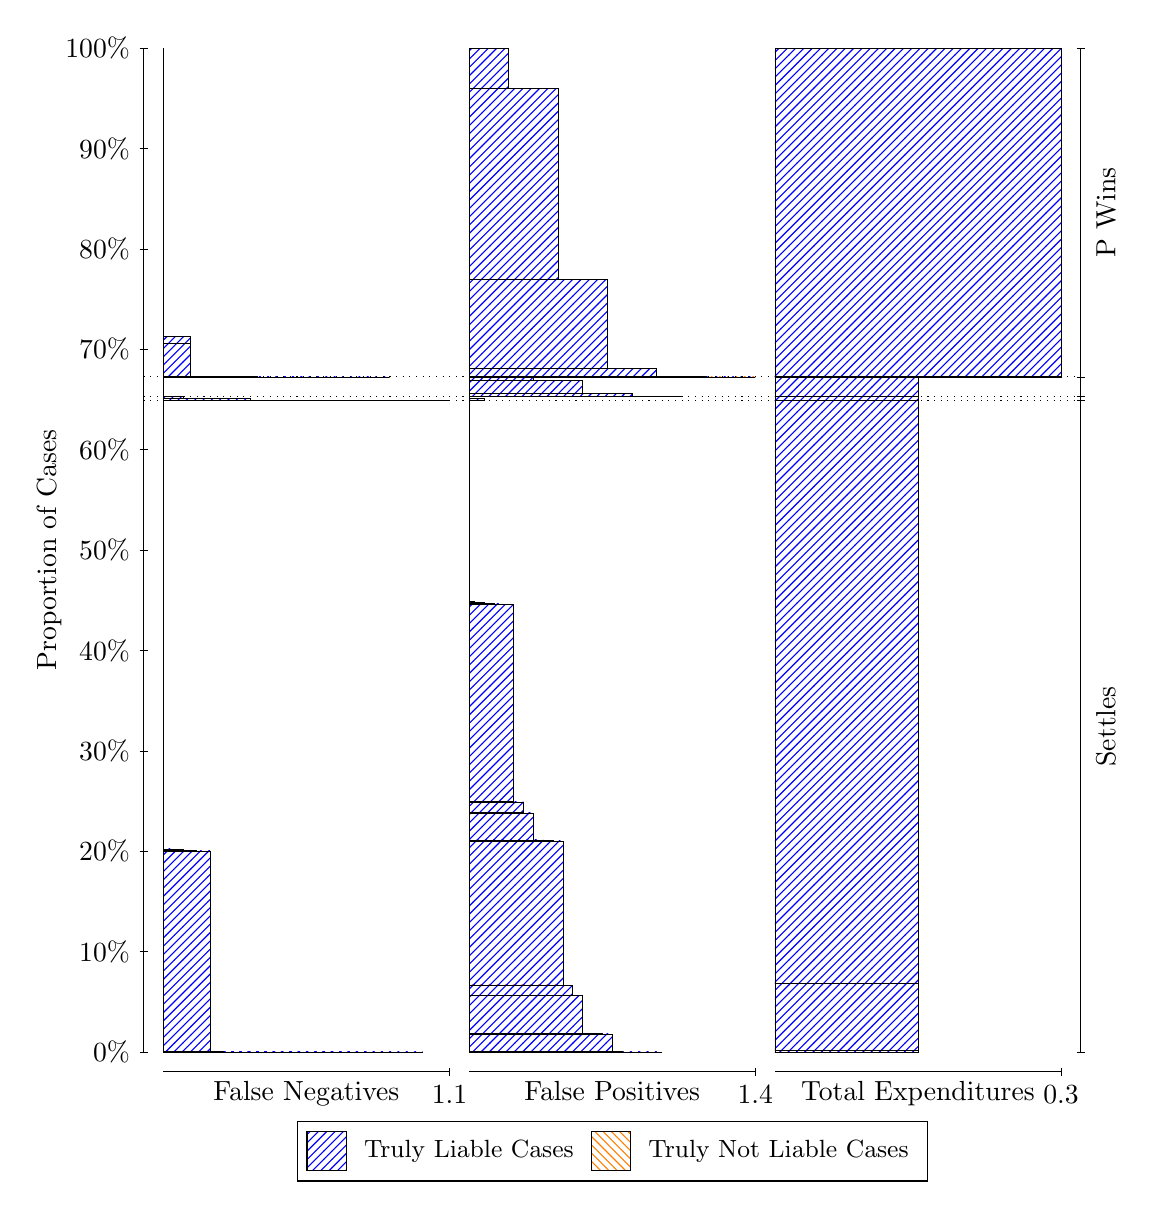
\begin{tikzpicture}
\draw[black, very thin] (1.5,1.75) -- (1.5,14.5);
\node[rotate=90, anchor=center] at (0.3, 8.125) {Proportion of Cases};
\draw[black, very thin] (1.45,1.75) -- (1.55,1.75);
\node[anchor=east] at (1.45, 1.75) {0\%};
\draw[black, very thin] (1.45,3.025) -- (1.55,3.025);
\node[anchor=east] at (1.45, 3.025) {10\%};
\draw[black, very thin] (1.45,4.3) -- (1.55,4.3);
\node[anchor=east] at (1.45, 4.3) {20\%};
\draw[black, very thin] (1.45,5.575) -- (1.55,5.575);
\node[anchor=east] at (1.45, 5.575) {30\%};
\draw[black, very thin] (1.45,6.85) -- (1.55,6.85);
\node[anchor=east] at (1.45, 6.85) {40\%};
\draw[black, very thin] (1.45,8.125) -- (1.55,8.125);
\node[anchor=east] at (1.45, 8.125) {50\%};
\draw[black, very thin] (1.45,9.4) -- (1.55,9.4);
\node[anchor=east] at (1.45, 9.4) {60\%};
\draw[black, very thin] (1.45,10.675) -- (1.55,10.675);
\node[anchor=east] at (1.45, 10.675) {70\%};
\draw[black, very thin] (1.45,11.95) -- (1.55,11.95);
\node[anchor=east] at (1.45, 11.95) {80\%};
\draw[black, very thin] (1.45,13.225) -- (1.55,13.225);
\node[anchor=east] at (1.45, 13.225) {90\%};
\draw[black, very thin] (1.45,14.5) -- (1.55,14.5);
\node[anchor=east] at (1.45, 14.5) {100\%};

\draw[black, very thin] (13.4,1.75) -- (13.4,14.5);
\draw[black, very thin] (13.35,1.75) -- (13.45,1.75);
\node[anchor=west] at (13.35, 1.75) {};
\draw[black, very thin] (13.35,10.021) -- (13.45,10.021);
\node[anchor=west] at (13.35, 10.021) {};
\draw[black, very thin] (13.35,10.079) -- (13.45,10.079);
\node[anchor=west] at (13.35, 10.079) {};
\draw[black, very thin] (13.35,10.323) -- (13.45,10.323);
\node[anchor=west] at (13.35, 10.323) {};
\draw[black, very thin] (13.35,14.5) -- (13.45,14.5);
\node[anchor=west] at (13.35, 14.5) {};

\draw[black, very thin, pattern color=blue, pattern=north east lines] (1.75,1.75) rectangle (5.0453,1.75);
\draw[black, very thin, pattern color=blue, pattern=north east lines] (1.75,1.75) rectangle (4.7074,1.75);
\draw[black, very thin, pattern color=blue, pattern=north east lines] (1.75,1.75) rectangle (4.3694,1.75);
\draw[black, very thin, pattern color=blue, pattern=north east lines] (1.75,1.75) rectangle (4.2004,1.75);
\draw[black, very thin, pattern color=blue, pattern=north east lines] (1.75,1.75) rectangle (4.0314,1.75);
\draw[black, very thin, pattern color=blue, pattern=north east lines] (1.75,1.75) rectangle (3.8624,1.75);
\draw[black, very thin, pattern color=blue, pattern=north east lines] (1.75,1.75) rectangle (3.6934,1.75);
\draw[black, very thin, pattern color=blue, pattern=north east lines] (1.75,1.75) rectangle (3.5244,1.75);
\draw[black, very thin, pattern color=blue, pattern=north east lines] (1.75,1.75) rectangle (3.3554,1.7501);
\draw[black, very thin, pattern color=blue, pattern=north east lines] (1.75,1.7501) rectangle (3.1864,1.7501);
\draw[black, very thin, pattern color=blue, pattern=north east lines] (1.75,1.7501) rectangle (3.1864,1.7501);
\draw[black, very thin, pattern color=blue, pattern=north east lines] (1.75,1.7501) rectangle (3.0174,1.7503);
\draw[black, very thin, pattern color=blue, pattern=north east lines] (1.75,1.7503) rectangle (2.8484,1.7503);
\draw[black, very thin, pattern color=blue, pattern=north east lines] (1.75,1.7503) rectangle (2.6795,1.7506);
\draw[black, very thin, pattern color=blue, pattern=north east lines] (1.75,1.7506) rectangle (2.6795,1.7506);
\draw[black, very thin, pattern color=blue, pattern=north east lines] (1.75,1.7506) rectangle (2.5105,1.7532);
\draw[black, very thin, pattern color=blue, pattern=north east lines] (1.75,1.7532) rectangle (2.3415,1.7533);
\draw[black, very thin, pattern color=blue, pattern=north east lines] (1.75,1.7533) rectangle (2.3415,1.7535);
\draw[black, very thin, pattern color=blue, pattern=north east lines] (1.75,1.7535) rectangle (2.3415,4.303);
\draw[black, very thin, pattern color=blue, pattern=north east lines] (1.75,4.303) rectangle (2.1725,4.307);
\draw[black, very thin, pattern color=blue, pattern=north east lines] (1.75,4.307) rectangle (2.0035,4.3238);
\draw[black, very thin, pattern color=blue, pattern=north east lines] (1.75,4.3238) rectangle (1.8345,4.3303);
\draw[black, very thin, pattern color=blue, pattern=north east lines] (1.75,4.3303) rectangle (1.8345,4.3303);
\draw[black, very thin, pattern color=orange, pattern=north west lines] (1.75,4.3303) rectangle (1.75,4.3303);
\draw[black, very thin, pattern color=blue, pattern=north east lines] (1.75,4.3303) rectangle (1.75,10.021);
\draw[black, very thin, pattern color=blue, pattern=north east lines] (1.75,10.021) rectangle (5.3833,10.021);
\draw[black, very thin, pattern color=blue, pattern=north east lines] (1.75,10.021) rectangle (4.5384,10.021);
\draw[black, very thin, pattern color=blue, pattern=north east lines] (1.75,10.021) rectangle (3.6934,10.022);
\draw[black, very thin, pattern color=blue, pattern=north east lines] (1.75,10.022) rectangle (2.8484,10.054);
\draw[black, very thin, pattern color=blue, pattern=north east lines] (1.75,10.054) rectangle (2.0035,10.079);
\draw[black, very thin, pattern color=orange, pattern=north west lines] (1.75,10.079) rectangle (1.75,10.079);
\draw[black, very thin, pattern color=blue, pattern=north east lines] (1.75,10.079) rectangle (2.0035,10.08);
\draw[black, very thin, pattern color=orange, pattern=north west lines] (1.75,10.08) rectangle (1.75,10.08);
\draw[black, very thin, pattern color=blue, pattern=north east lines] (1.75,10.08) rectangle (1.75,10.323);
\draw[black, very thin, pattern color=blue, pattern=north east lines] (1.75,10.323) rectangle (4.6229,10.323);
\draw[black, very thin, pattern color=blue, pattern=north east lines] (1.75,10.323) rectangle (3.7779,10.323);
\draw[black, very thin, pattern color=blue, pattern=north east lines] (1.75,10.323) rectangle (2.9329,10.332);
\draw[black, very thin, pattern color=blue, pattern=north east lines] (1.75,10.332) rectangle (2.088,10.745);
\draw[black, very thin, pattern color=blue, pattern=north east lines] (1.75,10.745) rectangle (2.088,10.836);
\draw[black, very thin, pattern color=orange, pattern=north west lines] (1.75,10.836) rectangle (1.75,10.836);
\draw[black, very thin, pattern color=blue, pattern=north east lines] (1.75,10.836) rectangle (1.75,14.5);
\draw[black, very thin, pattern color=orange, pattern=north west lines] (5.6333,1.75) rectangle (8.0764,1.75);
\draw[black, very thin, pattern color=blue, pattern=north east lines] (5.6333,1.75) rectangle (8.0764,1.7521);
\draw[black, very thin, pattern color=orange, pattern=north west lines] (5.6333,1.7521) rectangle (7.8259,1.7521);
\draw[black, very thin, pattern color=blue, pattern=north east lines] (5.6333,1.7521) rectangle (7.8259,1.7521);
\draw[black, very thin, pattern color=orange, pattern=north west lines] (5.6333,1.7521) rectangle (7.5753,1.7521);
\draw[black, very thin, pattern color=blue, pattern=north east lines] (5.6333,1.7521) rectangle (7.5753,1.7537);
\draw[black, very thin, pattern color=blue, pattern=north east lines] (5.6333,1.7537) rectangle (7.45,1.9806);
\draw[black, very thin, pattern color=orange, pattern=north west lines] (5.6333,1.9806) rectangle (7.3247,1.9806);
\draw[black, very thin, pattern color=blue, pattern=north east lines] (5.6333,1.9806) rectangle (7.3247,1.982);
\draw[black, very thin, pattern color=blue, pattern=north east lines] (5.6333,1.982) rectangle (7.1994,1.9836);
\draw[black, very thin, pattern color=orange, pattern=north west lines] (5.6333,1.9836) rectangle (7.0741,1.9836);
\draw[black, very thin, pattern color=blue, pattern=north east lines] (5.6333,1.9836) rectangle (7.0741,2.4662);
\draw[black, very thin, pattern color=blue, pattern=north east lines] (5.6333,2.4662) rectangle (6.9489,2.5991);
\draw[black, very thin, pattern color=orange, pattern=north west lines] (5.6333,2.5991) rectangle (6.8236,2.5991);
\draw[black, very thin, pattern color=blue, pattern=north east lines] (5.6333,2.5991) rectangle (6.8236,2.6022);
\draw[black, very thin, pattern color=orange, pattern=north west lines] (5.6333,2.6022) rectangle (6.8236,2.6022);
\draw[black, very thin, pattern color=blue, pattern=north east lines] (5.6333,2.6022) rectangle (6.8236,4.4308);
\draw[black, very thin, pattern color=blue, pattern=north east lines] (5.6333,4.4308) rectangle (6.6983,4.4378);
\draw[black, very thin, pattern color=orange, pattern=north west lines] (5.6333,4.4378) rectangle (6.573,4.4378);
\draw[black, very thin, pattern color=blue, pattern=north east lines] (5.6333,4.4378) rectangle (6.573,4.4448);
\draw[black, very thin, pattern color=blue, pattern=north east lines] (5.6333,4.4448) rectangle (6.4477,4.7877);
\draw[black, very thin, pattern color=orange, pattern=north west lines] (5.6333,4.7877) rectangle (6.3224,4.7877);
\draw[black, very thin, pattern color=blue, pattern=north east lines] (5.6333,4.7877) rectangle (6.3224,4.7898);
\draw[black, very thin, pattern color=blue, pattern=north east lines] (5.6333,4.7898) rectangle (6.3224,4.9252);
\draw[black, very thin, pattern color=blue, pattern=north east lines] (5.6333,4.9252) rectangle (6.1971,4.9291);
\draw[black, very thin, pattern color=blue, pattern=north east lines] (5.6333,4.9291) rectangle (6.1971,7.4335);
\draw[black, very thin, pattern color=orange, pattern=north west lines] (5.6333,7.4335) rectangle (6.0718,7.4335);
\draw[black, very thin, pattern color=blue, pattern=north east lines] (5.6333,7.4335) rectangle (6.0718,7.4355);
\draw[black, very thin, pattern color=blue, pattern=north east lines] (5.6333,7.4355) rectangle (6.0718,7.4403);
\draw[black, very thin, pattern color=blue, pattern=north east lines] (5.6333,7.4403) rectangle (5.9466,7.4469);
\draw[black, very thin, pattern color=blue, pattern=north east lines] (5.6333,7.4469) rectangle (5.8213,7.4636);
\draw[black, very thin, pattern color=blue, pattern=north east lines] (5.6333,7.4636) rectangle (5.696,7.4662);
\draw[black, very thin, pattern color=blue, pattern=north east lines] (5.6333,7.4662) rectangle (5.696,7.4677);
\draw[black, very thin, pattern color=blue, pattern=north east lines] (5.6333,7.4677) rectangle (5.6333,10.021);
\draw[black, very thin, pattern color=orange, pattern=north west lines] (5.6333,10.021) rectangle (5.8213,10.021);
\draw[black, very thin, pattern color=blue, pattern=north east lines] (5.6333,10.021) rectangle (5.8213,10.046);
\draw[black, very thin, pattern color=blue, pattern=north east lines] (5.6333,10.046) rectangle (5.6333,10.079);
\draw[black, very thin, pattern color=orange, pattern=north west lines] (5.6333,10.079) rectangle (8.327,10.079);
\draw[black, very thin, pattern color=blue, pattern=north east lines] (5.6333,10.079) rectangle (8.327,10.08);
\draw[black, very thin, pattern color=blue, pattern=north east lines] (5.6333,10.08) rectangle (7.7006,10.112);
\draw[black, very thin, pattern color=blue, pattern=north east lines] (5.6333,10.112) rectangle (7.0741,10.282);
\draw[black, very thin, pattern color=blue, pattern=north east lines] (5.6333,10.282) rectangle (6.4477,10.323);
\draw[black, very thin, pattern color=blue, pattern=north east lines] (5.6333,10.323) rectangle (5.8213,10.323);
\draw[black, very thin, pattern color=orange, pattern=north west lines] (5.6333,10.323) rectangle (9.2667,10.323);
\draw[black, very thin, pattern color=blue, pattern=north east lines] (5.6333,10.323) rectangle (9.2667,10.323);
\draw[black, very thin, pattern color=orange, pattern=north west lines] (5.6333,10.323) rectangle (8.6402,10.323);
\draw[black, very thin, pattern color=blue, pattern=north east lines] (5.6333,10.323) rectangle (8.6402,10.325);
\draw[black, very thin, pattern color=orange, pattern=north west lines] (5.6333,10.325) rectangle (8.0138,10.325);
\draw[black, very thin, pattern color=blue, pattern=north east lines] (5.6333,10.325) rectangle (8.0138,10.434);
\draw[black, very thin, pattern color=orange, pattern=north west lines] (5.6333,10.434) rectangle (7.3874,10.434);
\draw[black, very thin, pattern color=blue, pattern=north east lines] (5.6333,10.434) rectangle (7.3874,11.561);
\draw[black, very thin, pattern color=orange, pattern=north west lines] (5.6333,11.561) rectangle (6.7609,11.561);
\draw[black, very thin, pattern color=blue, pattern=north east lines] (5.6333,11.561) rectangle (6.7609,13.987);
\draw[black, very thin, pattern color=blue, pattern=north east lines] (5.6333,13.987) rectangle (6.1345,14.491);
\draw[black, very thin, pattern color=blue, pattern=north east lines] (5.6333,14.491) rectangle (5.6333,14.5);
\draw[black, very thin, pattern color=orange, pattern=north west lines] (9.5167,1.75) rectangle (11.333,1.75);
\draw[black, very thin, pattern color=blue, pattern=north east lines] (9.5167,1.75) rectangle (11.333,1.7742);
\draw[black, very thin, pattern color=orange, pattern=north west lines] (9.5167,1.7742) rectangle (11.333,1.7742);
\draw[black, very thin, pattern color=blue, pattern=north east lines] (9.5167,1.7742) rectangle (11.333,2.6213);
\draw[black, very thin, pattern color=orange, pattern=north west lines] (9.5167,2.6213) rectangle (11.333,2.6213);
\draw[black, very thin, pattern color=blue, pattern=north east lines] (9.5167,2.6213) rectangle (11.333,10.021);
\draw[black, very thin, pattern color=orange, pattern=north west lines] (9.5167,10.021) rectangle (11.333,10.021);
\draw[black, very thin, pattern color=blue, pattern=north east lines] (9.5167,10.021) rectangle (11.333,10.079);
\draw[black, very thin, pattern color=orange, pattern=north west lines] (9.5167,10.079) rectangle (11.333,10.079);
\draw[black, very thin, pattern color=blue, pattern=north east lines] (9.5167,10.079) rectangle (11.333,10.323);
\draw[black, very thin, pattern color=orange, pattern=north west lines] (9.5167,10.323) rectangle (13.15,10.323);
\draw[black, very thin, pattern color=blue, pattern=north east lines] (9.5167,10.323) rectangle (13.15,10.334);
\draw[black, very thin, pattern color=orange, pattern=north west lines] (9.5167,10.334) rectangle (13.15,10.334);
\draw[black, very thin, pattern color=blue, pattern=north east lines] (9.5167,10.334) rectangle (13.15,14.5);
\draw[black, dotted] (1.5,10.021) -- (13.4,10.021);
\draw[black, dotted] (1.5,10.079) -- (13.4,10.079);
\draw[black, dotted] (1.5,10.323) -- (13.4,10.323);
\draw[black, very thin] (1.75,1.5) -- (5.3833,1.5);
\node[anchor=north] at (3.5667, 1.5) {False Negatives};
\draw[black, very thin] (5.3833,1.45) -- (5.3833,1.55);
\node[anchor=north] at (5.3833, 1.45) {1.1};

\draw[black, very thin] (5.6333,1.5) -- (9.2667,1.5);
\node[anchor=north] at (7.45, 1.5) {False Positives};
\draw[black, very thin] (9.2667,1.45) -- (9.2667,1.55);
\node[anchor=north] at (9.2667, 1.45) {1.4};

\draw[black, very thin] (9.5167,1.5) -- (13.15,1.5);
\node[anchor=north] at (11.333, 1.5) {Total Expenditures};
\draw[black, very thin] (13.15,1.45) -- (13.15,1.55);
\node[anchor=north] at (13.15, 1.45) {0.3};

\node[black, centered, rotate=90] at (13.72, 5.8853) {Settles};


\node[black, centered, rotate=90] at (13.72, 12.412) {P Wins};

\draw (7.449999999999999,1.5) node[draw=none] (baseCoordinate) {};
\begin{scope}[align=center]
        \matrix[scale=0.5, draw=black, below=0.5cm of baseCoordinate, nodes={draw}, column sep=0.1cm]{
            \node[rectangle, draw, minimum width=0.5cm, minimum height=0.5cm, pattern=north east lines, pattern color=blue] {}; &
            \node[draw=none, font=\small] (B) {Truly Liable Cases}; &
            \node[rectangle, draw, minimum width=0.5cm, minimum height=0.5cm, pattern=north west lines, pattern color=orange] {}; &
            \node[draw=none, font=\small] (B) {Truly Not Liable Cases}; \\
            };
\end{scope}

\end{tikzpicture}
\end{document}